\chapter{Design and Implementation}
%  (max 5 pages)

% Detailed description of the work done, at the level of design and at the level of implementation. Focus on the architecture and coordination aspects (processes and tuple spaces).

% As an introduction to the design, briefly explain what initial picture we had for the game/program. How did we visualize the game/networking before writing the code?
% 
% What parts of the Doom networking have we chosen? Why?
% 
% How are tuplespaces used and distributed?
% 
% Who acts on the tuple spaces?
% 
% Figures of the protocols! (squares with circles, like in albertos lectures)
% 
% How are the packages/classes configured in the project? Explain the hierachy and how it makes the program more flexible.
% 
% What information is sent back and forth and why? How is that accomplished?
% 

%The game we implemented is played in real-time. At the same time, we wanted a static menu where players could join and leave games at their own pace. This made it so we had two different requirements for the tuplespaces, leading to two different approaches in server-client communication through a tuplespace.


\section{Design}

The general game flow in the client applications is designed as follows: Firstly, a user performs a login through a welcome screen by submitting a username. When logged in, the user enters a lobby, where all available rooms and idle players are listed. A user can then either create a new room\footnote{See the glossary \ref{tab:glossary} for the definition.}, or join an existing one. While in the room, the world is rendered and the game is active.


\subsection{The lobby}
%Before entering the lobby, the player goes through the login screen. Here they have to choose a unique username and a server to join. After this, they get taken to the lobby screen, which acts as a hub before the players join or create games, or rooms as we have dubbed them.


% The lobby is a tuplespace
% All information is accessed through the lobby
% All requests are put in the lobby
% A request is only granted, if the server replies with an acknowledgement.

The lobby UI is defined by a tuplespace in the server, also called \texttt{lobby}. All information in the lobby UI is accessed through the \texttt{lobby} tuplespace. A request is placed in the \texttt{lobby} tuplespace and is only granted, if the server replies with an acknowledgement. Every action in the lobby is performed through requests, and an example is shown on the left in figure \ref{fig:Protocols}. The \texttt{lobby} is hosted and maintained by the server.

%If the player wishes to perform actions in the lobby, such as creating or joining a room, they need to send up a request for the action to be performed. The server then parses these commands, and either allows it to be performed or denies it. This authoritative approach allows for greater security regarding server-side data.

\begin{figure}
    \centering
    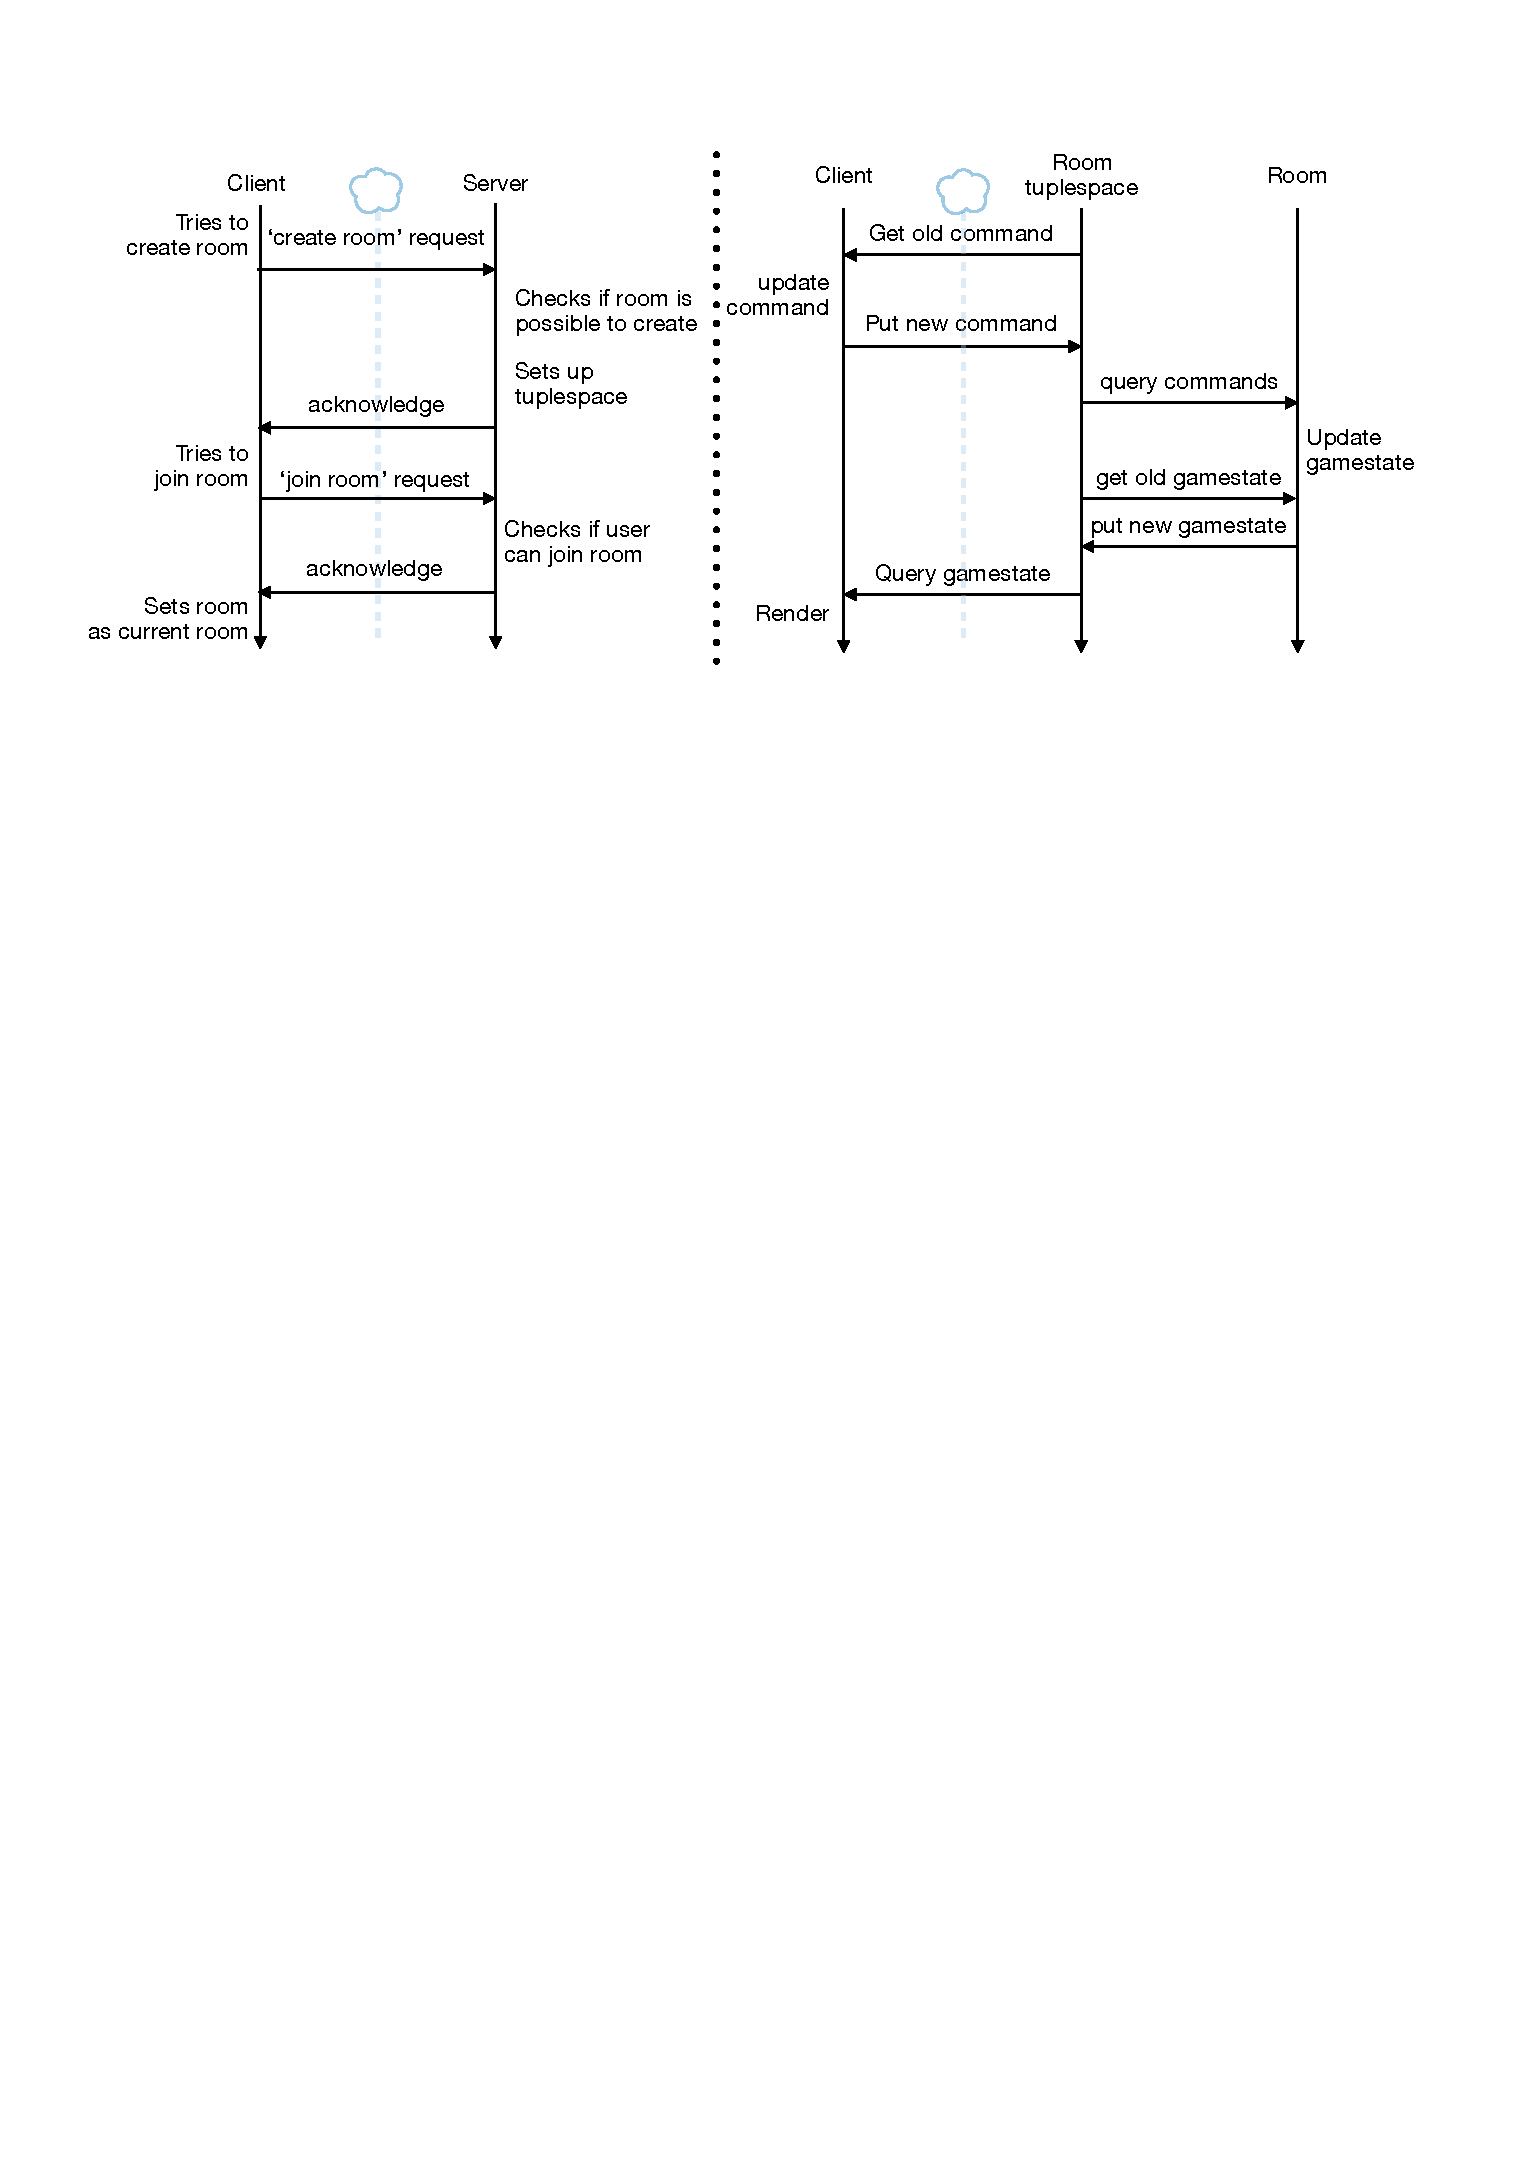
\includegraphics[width=\textwidth]{figures/Protocols.pdf}
    \caption{Protocols for the communication between client and server. Left) Client creates a room. Right) Updating the gamestate for a new frame. The remote communications are indicated by the cloud and the dotted line.}
    \label{fig:Protocols}
\end{figure}


\subsection{The game}

% A room is both a thread which updates a gamestate based on commands, and a tuple space
% Clients inform what inputs/commands are performed each frame 
% The room thread reads the commands from all players in the room and from that it updates the gamestate in the room tuplespace.
% Each frame, the clients read the current gamestate, and renders the players as specified in the gamestate. 
% A chat is also accessible between all players in a room, and the messages are placed in the room tuplespace to read.

Each game consists of a process, with a tuplespace, on the server. The process updates the gamestates\footnote{See the glossary \ref{tab:glossary} for the definition.} each frame and is called \texttt{room}. The \texttt{room} tuplespace contains all information necessary for that specific game. Each tick, the client informs what inputs/commands are performed, which the \texttt{room} process queries and uses to calculate the next gamestate. To render the game, the clients read the current gamestate and renders the players (including themselves) with the specified information, in the game UI. This exchange of information is seen on the right in figure \ref{fig:Protocols}. The interaction with the \texttt{room} tuplespace for the client and \texttt{room} process is independent of each other, making it possible to get all possible interleavings. This design ensures, that the \texttt{room} process is guaranteed the latest command from the user, and the user is guaranteed the latest gamestate from the \texttt{room} process.

In parallel to the game, a chat is updated, with the individual messages accessed through \texttt{room} tuplespace. As the tuplespace acts on a FIFO principle, the messages can be stored independently and still be queried in the correct order by the clients.

%The game itself was designed as a first-person shooter with 3D movement in real-time. This made us opt for a solution inspired by the network structure seen in the game Quake 3, described in section \ref{quake3source}. We did, however, go for a simplified approach. 

%The clients each send their commands to the server, which is read by the server-side program. The server updates the information about the game, which we dubbed the gamestate, according to the commands recieved from the clients. The gamestate contains information about every players position, rotation and any shots they may have fired, as well as their kills and deaths. The server then makes this information available to the clients. The clients render the game according to the new gamestate, and then the process repeats. Through this approach, no game logic is present in the client-side program.

%\footnote{Quake 3 Source Code Review: Network Model, by Fabien Sanglard: http://fabiensanglard.net/quake3/network.php}

% \begin{figure}[!h]
%     \centering
%     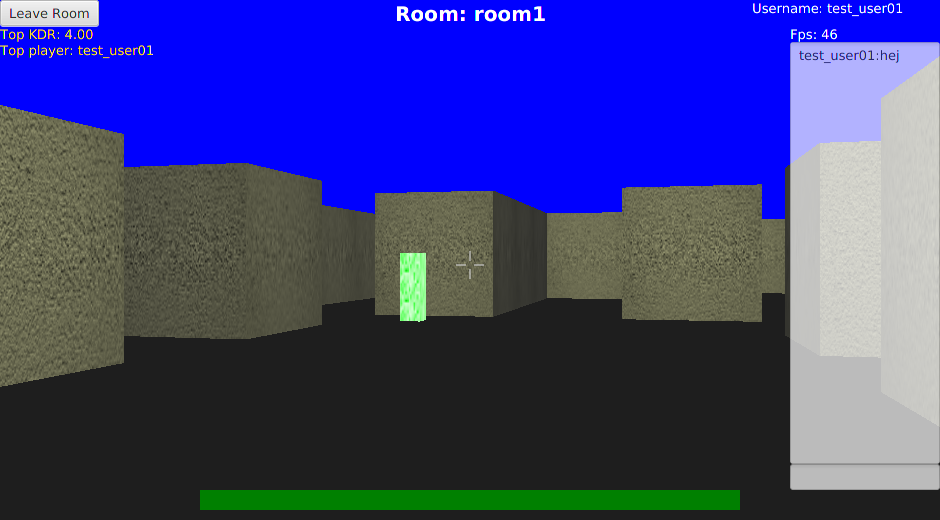
\includegraphics[scale=.3]{figures/room.png}
%     \caption{A picture of the window when in-game. The chat on the right side of the screen can be written to by players at any time. The green figure is another player. From the game, the player can leave the room by pressing the \textit{Leave room} at the top-left side of the screen.}
%     \label{fig:room}
% \end{figure}

%In addition to the game itself, we have a chat, wherein the players can talk among themselves in the current room. This information is sent independently of the gamestates, and is then always available to other clients.

In figure \ref{fig:CommunicationOverview} the communication between server and clients is visualized, where the interaction to the lobby is handled through the protocols defined in the class \texttt{MainConnector} and the interaction with the entered room/game is handled through the protocols defined in the class \texttt{RoomConnector}.

\begin{figure}[H]
    \centering
    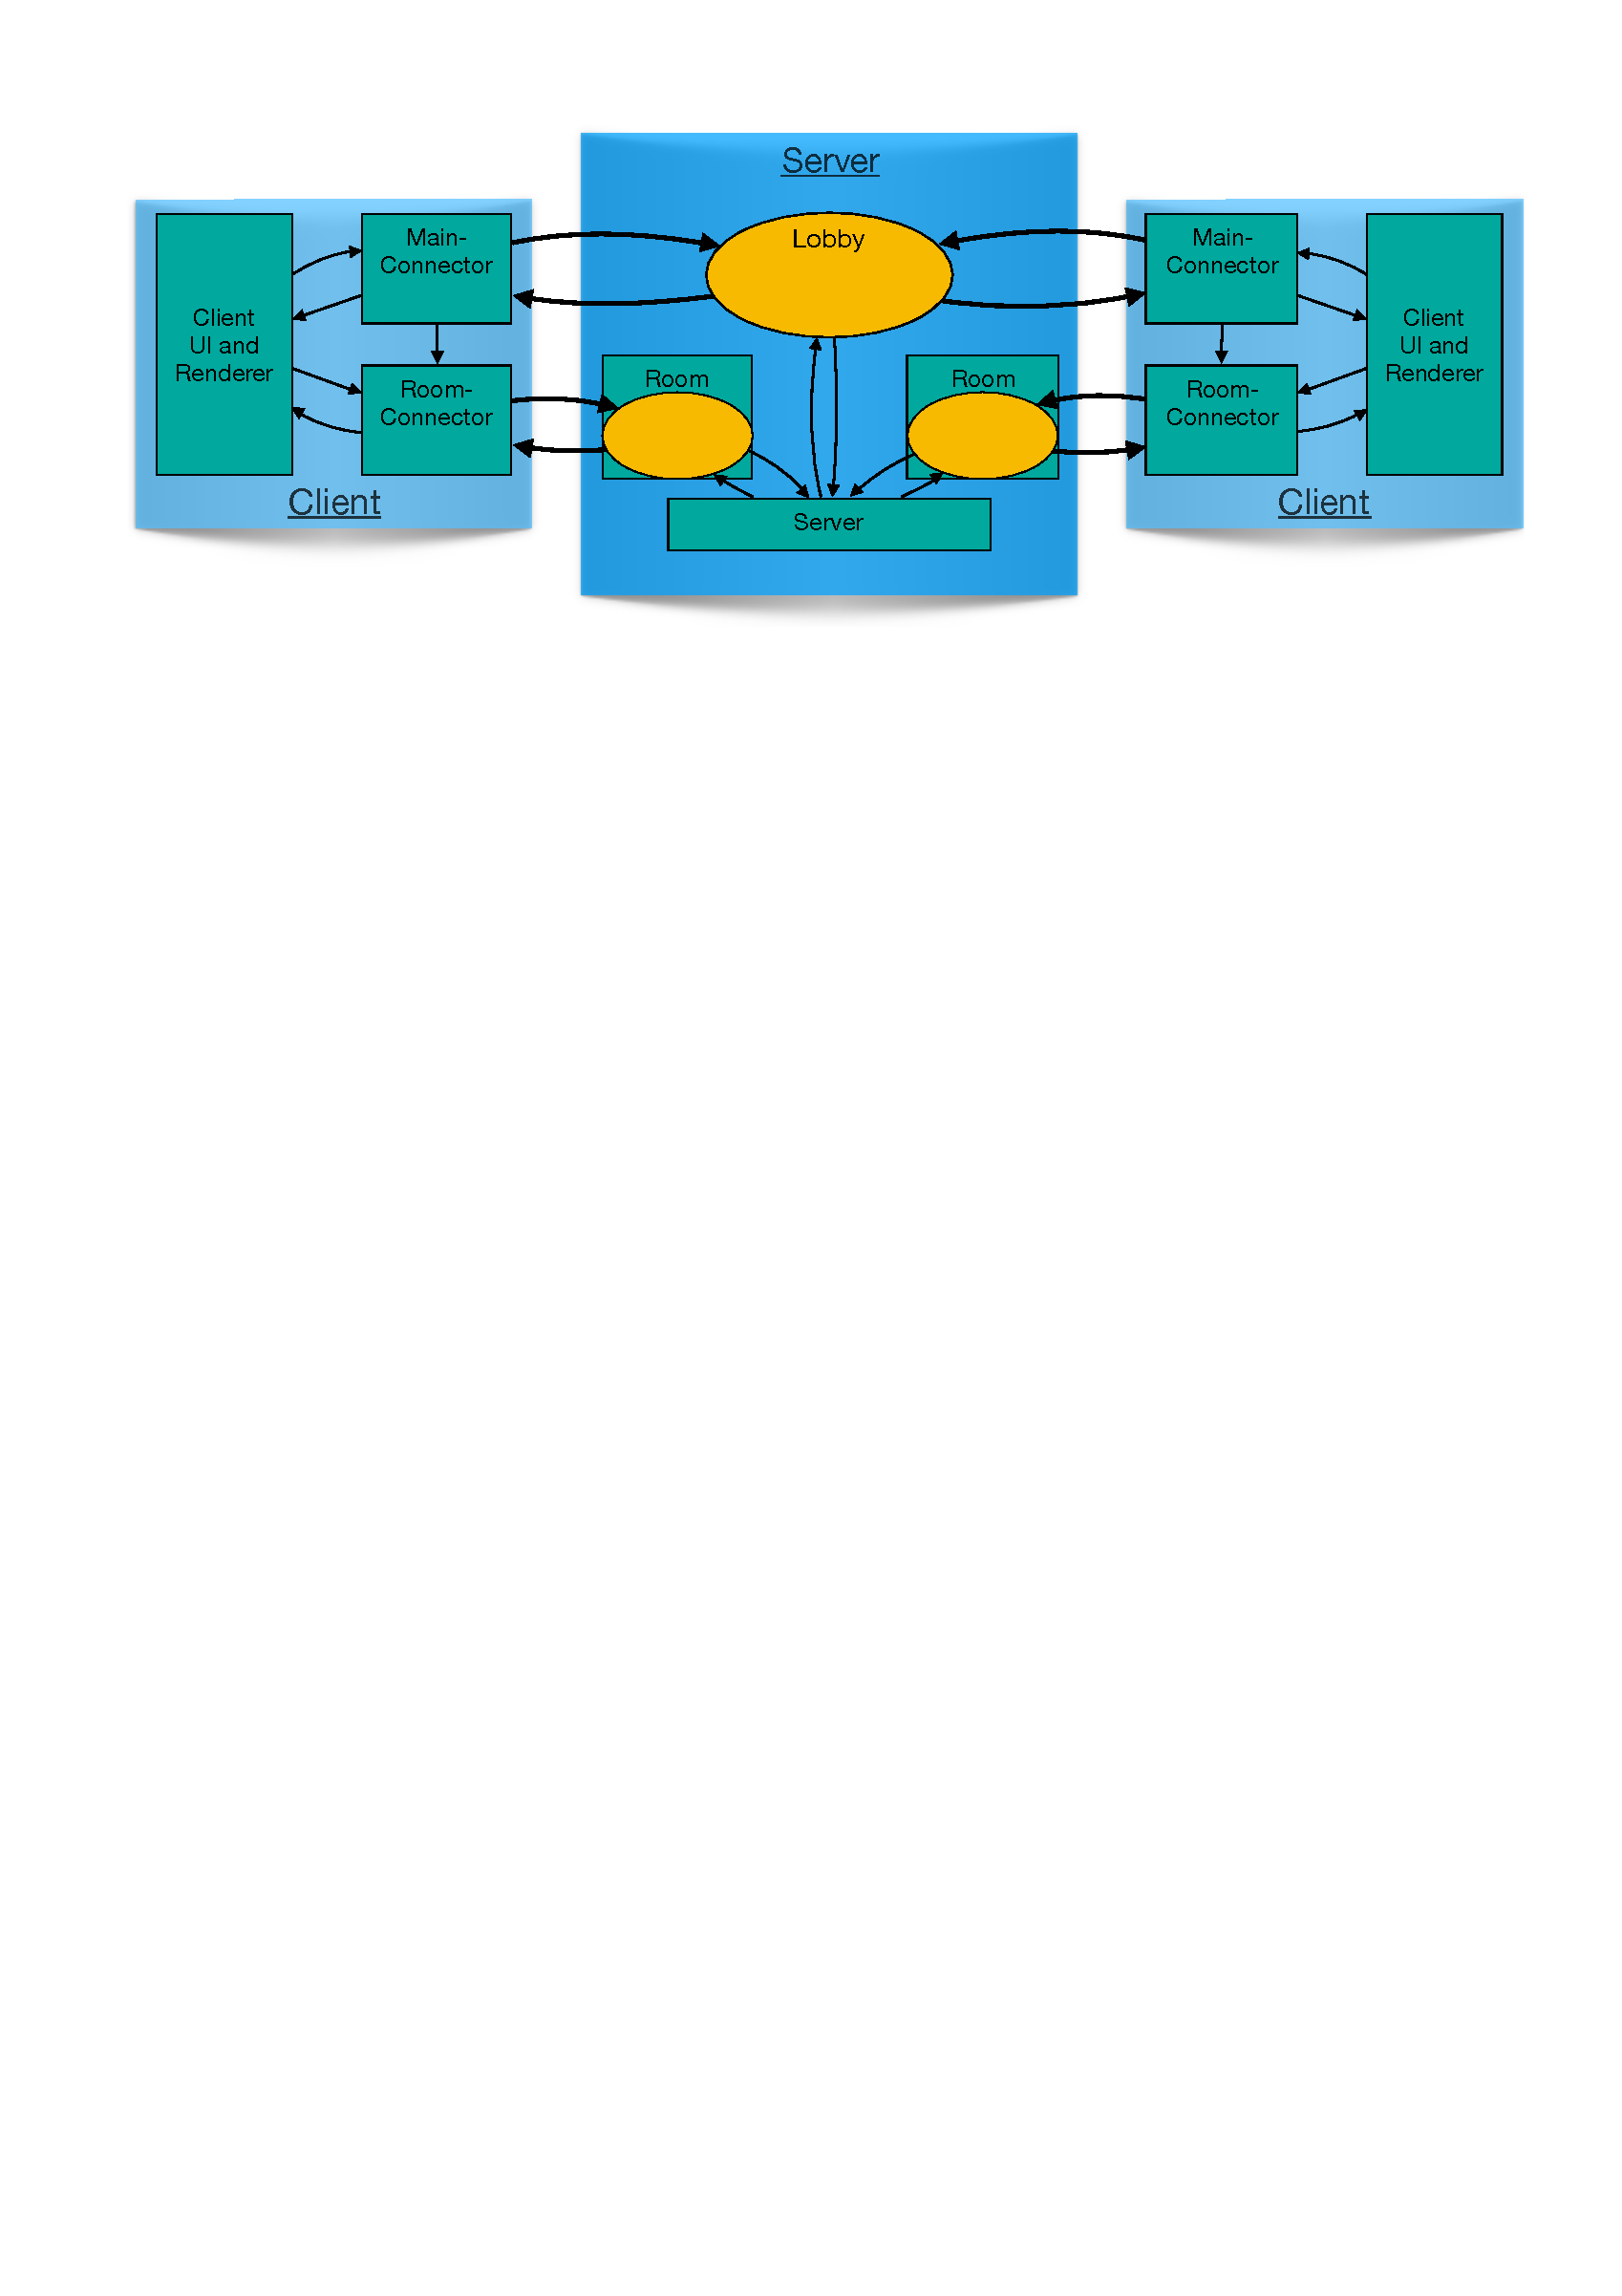
\includegraphics[width = \textwidth]{figures/CommunicationFigure.pdf}
    \caption{Communication between the server and clients. Devices are depicted as blue squares, tuplespaces as orange ovals and services as green squares. The information/communication flow is shown by the black arrows. Each Room service and tuplespace represents a different game, which clients can connect to. Here two games are running with a single client in each.}
    \label{fig:CommunicationOverview}
\end{figure}


\section{Implementation}

The implementations of the design choices are executed with respect to the challenges delineated in section \ref{sec:challenges}.

%\subsection{The lobby}

%The lobby tuplespace contains information regarding all rooms, players and commands the clients are trying to perform. The information is saved locally to the server, but is available in the tuplespace strictly so it can be looked up by the clients. 
%Commands are sent to the tuplespace from clients, and concern actions such as creating rooms, joining rooms etc. The server gets these, thus removing them from the tuplespace, and then runs a method to handle the command. If the command is allowed, the server handles the internal logic accordingly, and then sends an \texttt{ack} to the client through the tuplespace. If the command is disallowed, however, the server simply sends a \texttt{nack} to client to indicate the command was not performed. 

%\begin{figure}[!h]
%    \centering
%    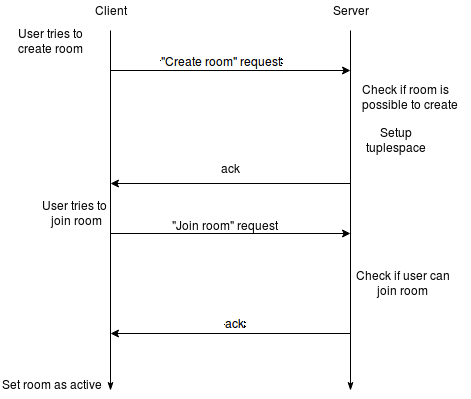
\includegraphics[scale=.5]{figures/lobby_comm.png}
%    \caption{An example of how the client communicates with the server. In this example, the user is trying to create a room. Note that the server and tuplespace have been combined in the figure, as the client and server are directly dependent on each others actions, and thus wait on each other during the process.}
%    \label{fig:lobby_comm}
%\end{figure}

%\subsection{The game}
%As the game works in real time, we opted for this to have its own separate tuple structure. Here, the clients send the commands input by the player once every tick of the game. This occurs whenever the client is done handling rendering of the previous gamestate, although it is capped to 60Hz. The server also updates once every tick, which happens with a rate of 60Hz. As the clients and server are not directly synchronized in tickrate, this means that the clients miss some gamestates. This is not much of a concern, as the gamestate contains all information, the clients can disregard any missed gamestates and simply update to the newest one and render. 

%For the chat, the tuple structure is a bit different, although it still acts within the same tuplespace as the game itself. For these, the client puts the messages into the tuplespace, which the other clients simply query the messages from the tuplespace. As these do not need to be regulated, and operate on a FIFO system, the messages can simply be queried directly from the tuplespace without going through the server itself, while still maintaining the correct order. 

%\begin{figure}[!h]
%    \centering
%    
\includegraphics[scale=.5]{figures/room_comm.png}
%    \caption{An example of how the client and server update their gamestates each tick of the server. Note that the client side and server side act independently of each other, and thus this is only one possible interleaving of many. This process repeats indefinitely.}
%    \label{fig:room_comm}
%\end{figure}

%\section{SPIN and security}

%Something something spin maybe?

\subsection{Classes and their responsibilities}
The final class diagram of \textsc{Team 10 Game} can be seen in figure \ref{fig:ClassesAndPackages}. In this section the most important classes, and their functionality, will be described briefly.

\begin{figure}
    \centering
    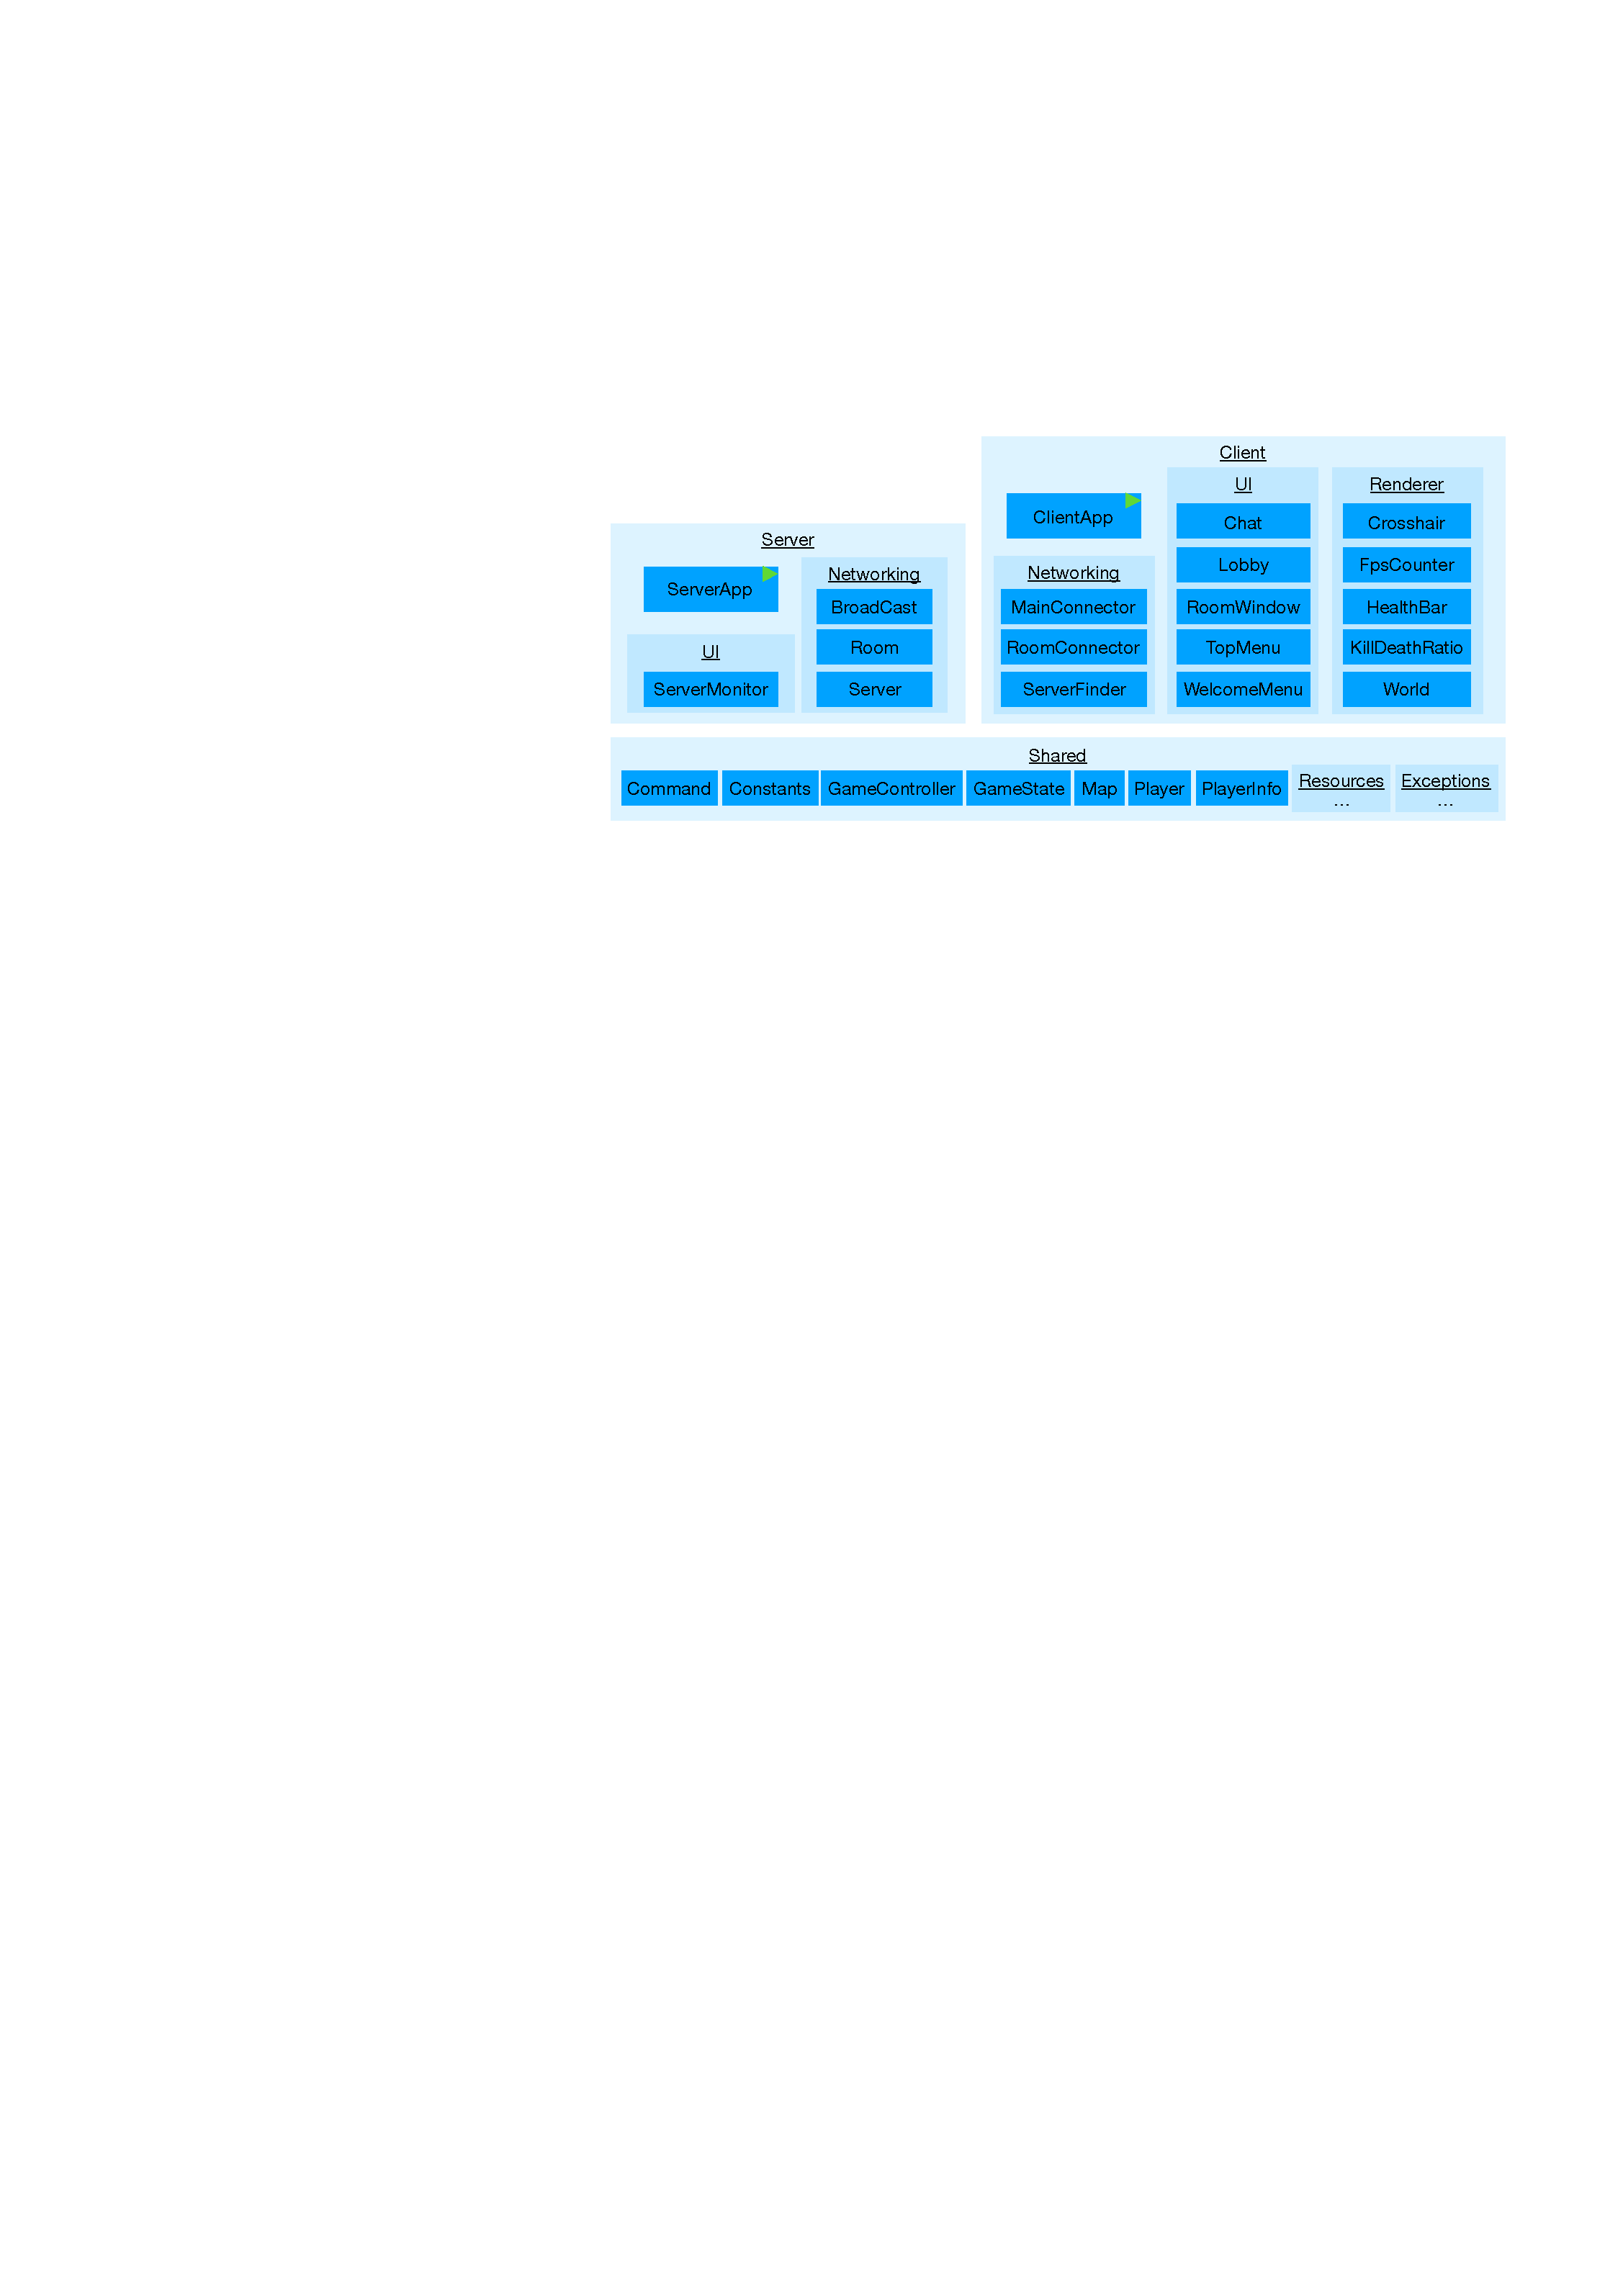
\includegraphics[width=\textwidth]{figures/ClassesAndPackages.pdf}
    \caption{The implemented classes in their respective packages for the complete project. Classes are depicted as blue squares, packages are semi-transparent squares.}
    \label{fig:ClassesAndPackages}
\end{figure}

\textbf{server: \texttt{server}}\\
The \texttt{server} class contains \texttt{static} methods and fields for running the server application. It has a \texttt{lobby} tuple space, a \texttt{SpaceRepository} and an \texttt{ArrayList<Room>} for dynamically allocating new game rooms. Its \texttt{handleRequest} method is continuously called to service clients waiting in the lobby. 

\textbf{server: \texttt{Room}}\\
\texttt{Room} \texttt{extends} \texttt{Sequential Space} and \texttt{implements} \texttt{Runnable}. This means that every instance of \texttt{Room} is itself hosting a tuple space and can be started as a new Java thread. This class holds top-level responsibility for maintaining and running a single game. It uses itself (as a tuple space) to \texttt{query} commands from all connected clients and \texttt{put}s a new game state every tick:
\vspace{-0.5cm}
\begin{center}
    \texttt{public void run () \{ while (true) \{ updateGamestate(); Thread.sleep(1000 / SERVER\_TICKRATE);\}\}}
\end{center}

\textbf{shared: \texttt{GameController}}\\
The \texttt{GameController} class holds all game-logic and rules. It contains 3 data structures: a \texttt{GameState}, a \texttt{Map} and a \texttt{List<Player>} on which it operates. Its most important method \texttt{applyCommands} takes a \texttt{List<Command>} and applies rules for all commands to its \texttt{GameState} which it returns. Each \texttt{Room} has a instance of \texttt{GameController} and calls \texttt{applyCommands} on every tick.  

\textbf{client: \texttt{MainConnector} \& \texttt{RoomConnector}}\\
The \texttt{MainConnector} and the \texttt{RoomConnector} both serve as mediators between the program and the server. The \texttt{MainConnector} handles communication related to the lobby, such as putting up requests and handling responses. As such, the \texttt{MainConnector} mostly consists of methods to be called by the \texttt{Lobby} UI whenever the user wishes to perform an action. The \texttt{RoomConnector} handles communication related to the rooms, and as such is mainly responsible for putting commands into the tuplespace and getting gamestates. These updates are executed through the \texttt{update} method, which is run every tick of the game by the \texttt{LobbyWindow} class.


\textbf{client: \texttt{World}}\\
The \texttt{World} class is the class responsible for rendering the game on the client-side of the program. 



\subsection{Data structures}
The main data structures of the implementation are tuplespaces and lists. Tuplespaces are used whenever a distributed data structure is needed, and lists are used for local storage, when data integrity is prioritized. An example of data integrity, is the gamestate in the \texttt{room} process. The new gamestate is calculated using the last master gamestate saved locally, and not the last gamestate from the \texttt{room} tuplespace. Any user can substitute this gamestate with custom information, and therefore may be dirty. This implementation ensures, that any breach in data integrity will be erased next frame. 

\textbf{Tuple patterns}\\
To implement the server/client protocols (such as those in figure \ref{fig:CommunicationOverview}) both sides has to agree upon how to pattern match in the tuplespace. This means that when the server \texttt{put}s a tuple to be read by the client, the client must know what abstract pattern to \texttt{query} or \texttt{get} - and vice versa with the server. Below on table \ref{tab:tuplepatterns} all the implemented tuple patterns can be seen. We settled with a "tag" method where each type of tuple has their first element as a static string to identify them. 

\begin{table}[htbp]
    \centering
    \begin{tabular}{rl}
    \textbf{Lobby Patterns} & \\
    \hline 
        Client id: & $(\texttt{"user"}, \texttt{String} : name)$  \\
        Room id: & $(\texttt{"room"}, \texttt{String} : name, \texttt{String} : owner)$
        \\
        Message: & $(\texttt{"message"}, \texttt{String} : user, \texttt{String} : msg)$
        \\
        Acknowledge: & $(\texttt{"response"}, \texttt{String} : user, \texttt{bool} : \texttt{true}/\texttt{false})$
        \\  
        Request: & $(\texttt{"createRoom"}, \texttt{String} : name, \texttt{String} : owner)$
        \\
        & $(\texttt{"joinRoom"}, \texttt{String} : name, \texttt{String} : user)$
        \\
        & $(\texttt{"leaveRoom"}, \texttt{String} : name)$
        \\
        & $(\texttt{"lockRoom"}, \texttt{String} : name, \texttt{String} : owner)$
        \\
        & $(\texttt{"quit"}, \texttt{String} : name, \texttt{String} : user)$
        \\
    \textbf{Room Patterns} & \\
    \hline
    Client id: & $(\texttt{String} : name)$  
    \\
    Message: & $(\texttt{"message"}, \texttt{String} : user, \texttt{String} : msg)$
    \\
    Command: & $(\texttt{"command"}, \texttt{String} : user, \texttt{Command} : cmd)$ 
    \\
    Game state: & $(\texttt{"gamestate"}, \texttt{GameState} : gs)$
    \\
    \end{tabular}
    \caption{The abstract tuple patterns used in \textsc{Team 10 Game}.}
    \label{tab:tuplepatterns}
\end{table}
